\documentclass[a4paper, 12pt]{article}
\usepackage[margin=1in]{geometry}
\usepackage{amsmath}
\setlength{\parindent}{0pt}
\usepackage{enumitem}
\usepackage{setspace}
% \setlist{itemsep=0pt,parsep=0pt}
\usepackage{url}
\usepackage{graphicx} % To include images
\usepackage{hyperref}   % To create hyperlinks
\addtolength{\parskip}{1ex}

\hypersetup{
    colorlinks=true,
    linkcolor=blue,
    filecolor=magenta,      
    urlcolor=cyan,
}

\usepackage{tikz}
\usetikzlibrary{
    shapes.multipart,
    positioning,
    arrows.meta
}

\title{A type-preserving compiler from a systems language to DTAL}
\author{Athena Eng}
\date{10 October 2025}

\begin{document}

\title{A type-preserving compiler from a systems language to DTAL}
\author{Athena Eng}
\date{10 October 2025}

\maketitle

\section{Introduction}

Systems programming languages such as C and C++ offer the programmer granular control over hardware and efficient use of resources, making them appropriate for performance-critical applications. However, these languages are fundamentally memory-unsafe and can lead to security vulnerabilities that go unnoticed in production code. For example, the Heartbleed bug \cite{CVE-2014-0160} was the result of an out-of-bounds read, which led to sensitive data being leaked.

There are several mechanisms that modern languages implement to address problems such as out-of-bounds access. Languages such as Python and Java use runtime checks and garbage collection to ensure memory safety guarantees, but these methods incur overhead that can degrade performance. The Rust programming language enforces compile-time safety using language features such as ownership and borrow-checking to prevent undefined behaviour (e.g. use-after-free and double free) that is prevalent in C and C++.

While Rust does provide a strong solution for preserving safety guarantees while maintaining performance comparable to C and C++, its correctness relies on the assumption that the compiler implementation is correct and preserves the semantics of the high-level (source) language. However, there may be situations in which a compiler for some given source language is not trusted. Projects such as CompCert \cite{compcert} and CakeML \cite{cakeml} have developed verified compilers that ensure compiled programs behave exactly as the source program was defined.

This dissertation project aims to move the locus of trust from the compiler to a simple, independent verifier. Formal compiler verification is complex and requires a lot of work whereas a verifier can be a small and simple trusted base. Proving the full semantic equivalence between source and target programs will be beyond the scope of this project. This project will implement a toolchain that uses type-preserving compilation to guarantee safety properties and statically verify the absence of certain unsafe behaviours and classes of runtime errors. A type-preserving compiler translates well-typed source code into verifiable target code, which for this project will be a typed assembly language. The typed assembly language will use features inspired by DTAL \cite{dtal}, where a register's type carries information about its value (e.g. the length of an array). Future work on this project could involve developing a formally verified compiler for the target assembly language such that both correctness and safety are achieved.

\subsection{Dependent Type Theory}

Dependent type theory (DTT) is a flavour of type theory that introduces dependent types, a type whose definition depends on a value. Dependent types also feature in Martin-L{\"o}f type theory, which can serve as an alternative foundation to mathematics. The theory promotes a view of a type as a mathematical proposition, where a value of that type would be a proof of that proposition. This correspondence between programs and proofs is known as the Curry-Howard isomorphism.

Type-checking DTT with extensional equality\footnote{extensional equality means that definitional equality is implied by propositional equality.} is actually undecidable. The work of Xi \& Pfenning, which was inspiration for this project, implements a dependently type assembly language (DTAL) using a restricted form of DTT based on the decidable logic of linear integer arithmetic. Types are not first-class citizens as one might observe in proof languages such as Agda, but rather exist at compile-time to verify program properties. This model allows the type system to be powerful enough to express properties like loop invariants and verify them statically. Using dependent types specifically enables certain compiler optimisations that would not be possible using a more traditional type system \cite{tal}. For example, runtime bounds checks can be transformed into compile-time proofs without the overhead.


\subsection{Safety Properties}

The dependent type system of this project is intended to provide a framework for proving program properties, with a focus on proving structural properties as described in the following.

\subsubsection*{Spatial Memory Safety}
\begin{itemize}
  \item Guarantee that every access to a memory buffer is within its legal bounds.
  \item We define an array's type as a dependent pair \texttt{(int, m)}, where \texttt{m} is the array's size. Any indexing operation generates a proof obligation (e.g. \texttt{0 <= i < m}), which must be solved by the compiler frontend.
\end{itemize}

\subsubsection*{Control-Flow Integrity}
\begin{itemize}
  \item Guarantee that branch instructions only target valid destinations.
  \item The DTAL labels destinations with a type to represent machine state, which will be compared with the current state at a branch instruction that jumps there, which involves subtype checking.
\end{itemize}

\subsubsection*{Integer Overflows}
\begin{itemize}
  \item Guarantees that integer arithmetic operations will not overflow or underflow.
  \item Range/refinement types can be used to guarantee integers stay within a range. These types can also be used for refining types in select blocks e.g. \texttt{\{i:int | i < 10\}}).
\end{itemize}

\subsubsection*{Preconditions and Postconditions}
\begin{itemize}
  \item Guarantees that a function is only ever called with inputs that satisfy given constraints.
  \item The HLL will have a language feature to specify preconditions (e.g. \texttt{require(m <= n)} on a function defines a $\Pi$-type). The compiler frontend then must prove this predicate holds true at every call.
\end{itemize}

The dependent type system could also be extended to prove more complex concurrent and behavioural properties. The following properties move beyond the core project.

\subsubsection*{Data Race Freedom}
\begin{itemize}
  \item Guarantees that two threads cannot concurrently access the same memory location if at least one of those accesses is a write.
  \item We could use ownership and linear/affine types similar to Rust's concurrency model and send and sync types for passing data between threads.
\end{itemize}

\subsubsection*{Information Flow Control}
\begin{itemize}
  \item Guarantees that sensitive information such as private keys and passwords cannot leak into public channels (e.g. log files, network sockets).
  \item We could extend the type system by incorporating security labels into the type system and define a security lattice that defines legal flow of information.
\end{itemize}

\subsubsection*{Communication Protocols}
\begin{itemize}
  \item Guarantees that two threads conform to a given message-passing protocol.
  \item Session types can be used for defining sequences of communication over a channel by describing the types that are expected to be sent/received during communication. Types evolve to reflect the next state of the protocol.
\end{itemize}

\section{Structure and Substance of the Project}

The core of this project will involve specifying a high-level systems language as the source language, low-level target language similar to DTAL as well as intermediate languages; implementation of a compiler for compiling the systems language to DTAL; and a verifier to assert a number of properties and safety guarantees in the generated target code.

Additional features that could build on the foundation of the core project include an interpreter for the generated DTAL, extending the specified core languages and support for concurrency properties and behavioural correctness. The full list of proposed extensions for the project are listed in 4.2.

The implementation will be written in Rust, which offers safety, stability and high performance.

\subsection{Main Components}

\autoref{fig:model} shows the components of the project and their inputs and outputs. The core components include specification of the source and target languages, the compiler and the verifier, whereas the assembler and linker for generating an object file from the DTAL will be an extension.

As stated in the introduction, the goal of this project is not to produce a formally verified compiler. Hence, in the design of this system, the compiler is untrusted, though compiler implemented in this project should perform the essential function of faithfully encoding the high-level safety specifications of the source language as explicit type annotations in the low-level code. The trusted component is the verifier, which will take the DTAL file as input and independently check that claims expressed in the type-annotated instructions logically follow from the code's execution. Hence, its correctness is paramount for providing a definite guarantee that programs are free from given classes of errors.

\begin{figure}[h!]
  \centering

  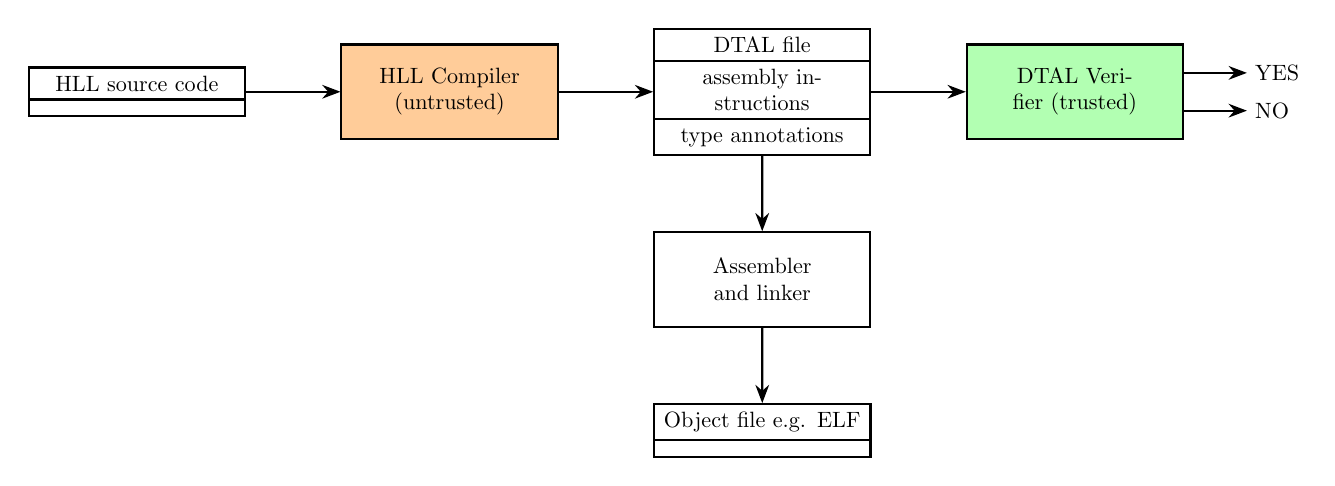
\begin{tikzpicture}[
      scale=0.8, transform shape,
      % Set distances between nodes
      node distance=1.2cm and 1.5cm,
      % Define styles for the elements
      base/.style={
          rectangle,
          draw,
          thick,
          text centered,
          minimum height=1.5cm,
          text width=3.2cm
        },
      untrusted/.style={
          base,
          fill=orange!40
        },
      trusted/.style={
          base,
          fill=green!30
        },
      multi/.style={
          base,
          rectangle split,
          rectangle split horizontal=false
        },
      arrow/.style={
          -Stealth, % Arrow tip style
          thick
        }
    ]

    % Place the nodes
    \node[multi, rectangle split parts=2] (hll) {
      HLL source code
      \nodepart{two}
    };

    \node[untrusted, right=of hll] (compiler) {
      HLL Compiler (untrusted)
    };

    \node[multi, rectangle split parts=3, right=of compiler] (dtal) {
      DTAL file
      \nodepart{two} assembly instructions
      \nodepart{three} type annotations
    };

    \node[trusted, right=of dtal] (verifier) {
      DTAL Verifier (trusted)
    };

    \node[base, below=of dtal] (assembler) {
      Assembler and linker
    };

    \node[multi, rectangle split parts=2, below=of assembler] (object_file) {
      Object file e.g. ELF
      \nodepart{two}
    };

    % Draw the arrows connecting the nodes
    \draw[arrow] (hll) -- (compiler);
    \draw[arrow] (compiler) -- (dtal);
    \draw[arrow] (dtal) -- (verifier);
    \draw[arrow] (dtal) -- (assembler);
    \draw[arrow] (assembler) -- (object_file);

    % Draw the 'YES' and 'NO' output arrows from the verifier
    \draw[arrow] ([yshift=0.3cm]verifier.east) -- ++(1,0) node[right] {YES};
    \draw[arrow] ([yshift=-0.3cm]verifier.east) -- ++(1,0) node[right] {NO};

  \end{tikzpicture}
  \caption{System model of the project}
  \label{fig:model}
\end{figure}



\subsubsection*{High-level Language Design}

The source language will be a minimal systems language (consisting of C-like and Rust-like features) focused on demonstrating the core safety properties.

\begin{itemize}
  \item Constructs:
    \begin{itemize}
      \item first-order functions (\texttt{fn})
      \item assignment (\texttt{let})
      \item if/else
      \item for (\texttt{for i in 0..n})
      \item preconditions (\texttt{requires(...)})
    \end{itemize}
  \item Types:
    \begin{itemize}
      \item primitive types (\texttt{int}, \texttt{bool})
      \item fixed-size array (\texttt{[T; N]}, where \texttt{T} is the element type and \texttt{N} is the size)
      \item immutable reference (\texttt{\&T})
      \item mutable variable (\texttt{let mut x = ...})
      \item singleton types (\texttt{int(c)})
      \item range/refinement types (\texttt{\{i: int | P(i)\}}, where \texttt{P} is some proposition)
    \end{itemize}
\end{itemize}

\subsubsection*{DTAL Design}

The target DTAL will be a RISC-like instruction set but every instruction will have a formal typing rule so it can be verified.

\paragraph{ISA:}
\begin{itemize}
  \item Moving data (\texttt{mov}, \texttt{load}, \texttt{store})
  \item Arithmetics (\texttt{add}, \texttt{sub}, \texttt{mul})
  \item Control flow (\texttt{jmp}, \texttt{cmp}, \texttt{blt}, \texttt{bgt}, \texttt{beq}, \texttt{ret})
\end{itemize}

\paragraph{Type system:}
\begin{itemize}
  \item primitive types
  \item dependent integer types
  \item pointer types (\texttt{ptr(T)})
  \item state types for labels (\texttt{r1:T1, ...})
  \item function types for entry points (\texttt{(args...) -> ret})
\end{itemize}

% The typing rules would then be used for type inference and assigning types e.g:
% \begin{itemize}
%   \item The instruction \texttt{load dest, [base, idx]} requires a proof that \texttt{0 <= idx < N}, where the register \texttt{base} has a type of a pointer to a fixed-size array, in order to assign \texttt{dest} with the type \texttt{T}.
% \end{itemize}

\subsubsection*{Compiler Frontend}

The first stage of the compiler frontend involves lexing and parsing, which will be done with the help of a parser generator/combinator to build an abstract syntax tree (AST). There are several existing Rust crates\footnote{A Rust crate is a compilation unit that the Rust compiler processes at a time e.g. binaries, libraries} that do this. The type-checker will the main substance of work for the frontend. It will traverse the AST and apply the language's formal typing rules as well as generating and solving proof obligations. For example:

\begin{itemize}
  \item For an array access \texttt{arr[i]}, the types of \texttt{arr} (e.g. \texttt{\&(int, m)}) and \texttt{i} are synthesised and the proof obligation \texttt{i >= 0 \&\& i < m} is generated.
  \item For a function with a \texttt{requires(n <= m)} clause, the function arguments are substituted into the clause to generate a proof obligation.
\end{itemize}

After the AST has been fully traversed, the frontend will have a set of logical constraints that must hold true. The constraint solving will be done with the help of an external SMT solver such as Z3. Finally, the AST will be annotated with the verified types. % [what annotation info?]

\subsubsection*{Compiler Backend}

The compiler backend is responsible for translating the AST from the frontend into a linear sequence of well-typed DTAL. Note that the compiler I develop will not be formally verified but it should perform proof transformations faithfully, encoding the safety guarantees verified by the frontend as correct and explicit type annotations in the target DTAL. The project's model assumes that the compiler could be incorrect, but the compiler delivered here aims to be as correct as possible by following standard engineering principles. Implementation will be semantics-driven with rigorous testing to maximise confidence of correctness.

The backend's workflow will be implemented as a multi-stage pipeline that will consist of:
\begin{itemize}
  \item Lowering to a defined typed intermediate representation (IR) that will resemble a linear, three-address code representation structured as a CFG using simplifying assumptions e.g. (an infinite set of virtual registers).
  \item Instruction selection and typed code generation where each instruction in the IR is mapped to one or more DTAL instructions. This process should preserve and encode type information.
  \item Typed register allocation where a register allocation algorithm will be implemented that takes the type system into account.
  \item Emission of DTAL file containing the finalised instructions with annotations and labels.
\end{itemize}

Some examples of transformations to DTAL include:

\begin{itemize}
  \item Arithmetic expression translation: we can derive resulting dependent types (e.g. for \texttt{add r3, r1, r2} where \texttt{r1:int(1)} and \texttt{r2:int(2)} the result register \texttt{r3} has type \texttt{int(3)}).
  \item Selection statement translation: we can generate explicit labels and conditional branch instructions. Refinement types can be used to refine the type of values in registers based on conditions (e.g. \texttt{r1:int} becomes \texttt{r1:\{i:int|i < 10\}} for a branch where the value in r1 $<$ 10).
  \item For loop translation: loop invariants can be expressed as a type (e.g. \texttt{r1:\{i:int|0 <= i < n\}}) and we can generate loop start/end labels.
\end{itemize}

\subsubsection*{DTAL Verifier}

The DTAL verifier will take the generated assembly and verify its proofs. This is the root of trust in the system so it should be small and simple (relative to the compiler). As mentioned, the compiler is large and complex whereas it is far more tractable to formally verify the verifier. This helps achieve a level of certified safety in contexts such as supply chain security or platform providers where there may zero trust in external toolchains.

The verifier will lex and parse the assembly to produce an AST for the DTAL grammar. From this, we build a control flow graph with annotated type information where each node is a basic block and the edges between blocks are the branch instructions. Using the CFG, we can execute an algorithm to perform data flow analysis that keeps track of the types of register values and prove that this is consistent with the type annotations. Some components and mechanisms used for the compiler frontend can be reused here e.g. verification of logical constraints via an SMT solver, AST traversal etc.

Within a block in the CFG, the verifier can perform actions on each instruction to check and update. For example, an instruction such as \texttt{mov r4, 0} will update the type state to express that \texttt{r4} is of the singleton type $\textsf{int}(0)$. For an instruction \texttt{load r3, [r1, r2]} where \texttt{r1} is a pointer to an array with type $\textsf{ptr}(\textsf{array}(\textsf{int}, m))$ and \texttt{r2} is an index \textsf{nat} to access the array, the algorithm would need to check \texttt{m} against proofs in the typing state to ensure that the value in \texttt{r2} is less than $m$.

Given that the verifier should be trusted, it will need to be rigorously tested. It is intended to be small enough such that a full manual audit would be possible. The gold standard would be formal verification via a proof assistant, which would be a major extension to the project.

\section{Starting Point}
\begin{itemize}
  \item The Part IB Compiler Construction, Introduction to Computer Architecture and Semantics of Programming Languages courses covered concepts relevant to this project.
  \item I have foundational knowledge of dependent type theory, having used it as the topic of an introductory technical talk I delivered.
  \item I have limited practical experience with proof-carrying code and using proof assistants.
  \item I do not have extensive practical experience with compiler development.
  \item I began learning the Rust programming language over the 2025 summer vacation and worked in a Rust codebase during my internship.
\end{itemize}

\section{Success Criterion}

\subsection{Core}

\begin{itemize}
  \item High-level language with core language features (see 2.1).
  \item DTAL with core language features (see 2.1). The extended version of Xi and Pfenning's paper \cite{dtal} contains the full rules of a DTAL, which can be used as reference.
  \item Compiler frontend to fully support lexing, parsing and type-checking of the core high-level language and its type system. There are existing type-checkers for refinement type systems that can be used from reference.
  \item Compiler backend to fully support compilation of the core high-level language and reject unsafe programs at compile time for the core safety properties (see 1.2).
  \item Verifier that accepts assembly code generated from safe programs.
\end{itemize}

\subsection{Extensions}

\begin{itemize}
  \item An interpreter and object file generator to produce an executable from the target DTAL.
  \item Support for modularised compilation, verification and linking.
  \item Widening the language and type system with more features (e.g. structs, generics, error handling, ownership, linear types).
  \item Prove some concurrency and behavioural correctness properties such that the verifier accepts a wider range of correct programs.
\end{itemize}

\section{Evaluation Plan and Metrics}

I will create a test suite to test the final system against safe and unsafe programs which should compile and verify, or be rejected by the DTAL verifier. With the language features defined in my core, this can write programs for performing calculations such as Fibonacci, factorial etc. and performing operations on vectors such as sorting. The Rust QuickCheck crate\footnote{https://docs.rs/quickcheck/latest/quickcheck/} can be used for generating programs with predefined properties to test the toolchain.

I will also measure end-to-end compilation time in order to evaluate to what extent ensuring correctness impacts performance. I will also perform a qualitative assessment of the range of safety properties that can be expressed or enforced by the language, and how this translates to its real-world application.


\section{Timetable and Milestones}

\subsection{Michaelmas Term}

\begin{itemize}
  \item \textbf{16 Oct. - 29 Oct.}
    \begin{itemize}
      \item Design and formally define core high-level language, DTAL and type system.
      \item \textbf{Milestone}: Send formal definition of semantics and typing rules of the HLL and DTAL to supervisor for review and beginnings of their in-code implementation.
    \end{itemize}
  \item \textbf{30 Oct. - 12 Nov.}
    \begin{itemize}
      \item Finish with design and implementation of languages.
      \item Implement lexer and parser (using parser generator/combinator).
      \item \textbf{Milestone}: Send full design of languages with lexer and parser for the HLL to supervisor for review.
    \end{itemize}
  \item \textbf{13 Nov. - 26 Nov.}
    \begin{itemize}
      \item Revision for DSP module written test.
      \item DSP module written test (21 Nov.)
      \item Start implementing frontend type-checker (if time allows).
      \item \textbf{Milestone}:
    \end{itemize}
  \item \textbf{27 Nov. - 10 Dec.}
    \begin{itemize}
      \item Implement the frontend type-checker with proof obligation checking using a logical constraint solver.
      \item \textbf{Milestone}: Implemented type-checker that applies formal typing rules with passing unit tests covering the major blocks of logic; compiler frontend implementation complete and ready for supervisor review.
    \end{itemize}
\end{itemize}


\subsection{Michaelmas Vacation}
\begin{itemize}
  \item \textbf{11 Dec. - 24 Dec.}
    \begin{itemize}
      \item Break
      \item Design IR and implement translation of HLL to IR.
      \item \textbf{Milestones}: Complete design of IR and translator.
    \end{itemize}
  \item \textbf{25 Dec. - 7 Jan.}
    \begin{itemize}
      \item Implement translation of IR to DTAL.
      \item \textbf{Milestones}: Complete translator that lowers IR to DTAL and preserves type information.
    \end{itemize}
  \item \textbf{8 Jan. - 21 Jan.}
    \begin{itemize}
      \item Implement register allocation algorithm.
      \item Implement emitter to output final DTAL code.
      \item \textbf{Milestone}: Majority of compiler backend implementation complete.
    \end{itemize}
\end{itemize}


\subsection{Lent Term}
\begin{itemize}
  \item \textbf{22 Jan. - 4 Feb.}
    \begin{itemize}
      \item Progress report and presentation.
      \item Start implementing verifier.
      \item \textbf{Milestones}: Delivered progress report and presentation and have beginnings of a verifier implementation (lexer, parser, CFG construction).
    \end{itemize}
  \item \textbf{5 Feb. - 18 Feb.}
    \begin{itemize}
      \item Plan structure of dissertation.
      \item Finish verifier implementation (data flow analysis logic)
      \item \textbf{Milestone}: Verifier implementation complete.
    \end{itemize}
  \item \textbf{19 Feb. - 3 Mar.}
    \begin{itemize}
      \item Write dissertation introduction.
      \item Begin end-to-end testing and evaluation.
      \item \textbf{Milestone}: Submit draft of dissertation to supervisor and obtain some evaluation results.
    \end{itemize}
  \item \textbf{4 Mar. - 17 Mar.}
    \begin{itemize}
      \item Write dissertation preparation section.
      \item Buffer time.
      \item \textbf{Milestone}: Submit draft of dissertation to supervisor.
    \end{itemize}
\end{itemize}

\subsection{Easter Vacation}
\begin{itemize}
  \item \textbf{18 Mar. - 31 Mar.}
    \begin{itemize}
      \item Write dissertation implementation section.
      \item Extensions
      \item \textbf{Milestone}: Submit draft of dissertation to supervisor.
    \end{itemize}
  \item \textbf{1 Apr. - 14 Apr.}
    \begin{itemize}
      \item Write dissertation evaluation section.
      \item Extensions
      \item \textbf{Milestone}: Submit full draft of dissertation to supervisor.
    \end{itemize}
  \item \textbf{15 Apr. - 28 Apr.}
    \begin{itemize}
      \item Work on drafts of dissertations.
      \item Extensions
      \item \textbf{Milestone}: Dissertation approved by supervisor.
    \end{itemize}
\end{itemize}

\subsection{Easter Term}
\begin{itemize}
  \item \textbf{29 Apr. - 10 May}
    \begin{itemize}
      \item Final checks.
      \item \textbf{Milestone}: Dissertation ready for submission.
    \end{itemize}
\end{itemize}

\section{Resources Declaration}

I will be developing on my laptop for this project. It has a 13th Gen Intel(R) Core(TM) i7-1365U processor and 32 GB RAM. I will make regular backups of the code to a private GitHub repository and a USB drive.

\ifdefined\maindoc
\else
\bibliographystyle{unsrt}
\bibliography{references}
\fi

\end{document}


